\documentclass[hyperref={pdfpagemode=FullScreen, colorlinks=false}]{beamer}

\usepackage{selinput}			% Inputencoding
	\SelectInputMappings{adieresis={ä}, germandbls={ß}, Euro={€}}
\usepackage[T1]{fontenc}		% Fontencoding
%
\usepackage{pifont}
\usepackage{csquotes,siunitx}			% Anführungszeichen; wird von biblatex gewünscht
\usepackage[backend=biber,citestyle=alphabetic,uniquelist=false]{biblatex}	% Literatur formatieren
\addbibresource{bodendynamik.bib}	% Literaturdatenbank
\usepackage{caption} 
\usepackage{subfig}
\usepackage{comment}
%%%%%%%%%%%%%%%%%%%%%%%%%%%%%%%%%%%%%%%%%%%%%%%%%%%%%%%%%%%%%%%%%%%%%%%%%%%%%%%%%%%%%%%%%%%%%%%%%%%%%%%
% Thema für Präsentation
\usetheme[fusszeile=ernstcolor,sprache=ngerman,seite=letzte,
verhaeltnis=16:10,
hausschrift=false,
navigation=false,
titelseite=blau]{TUBAF}

\TUBAFZweitlogo{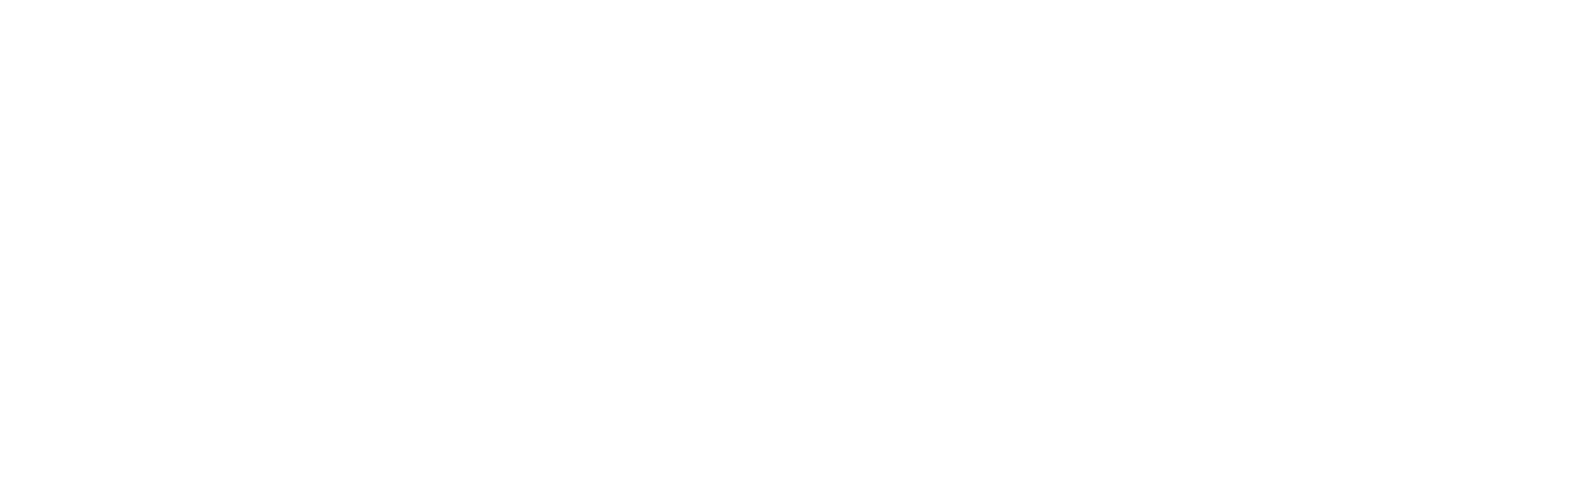
\includegraphics{fig_pdf/UFZ_logo_inv.pdf}}

%%%%%%%%%%%%%%%%%%%%%%%%%%%%%%%%%%%%%%%%%%%%%%%%%%%%%%%%%%%%%%%%%%%%%%%%%%%%%%%%%%%%%%%%%%%%%%%%%%%%%%%
% Optionen für Anmerkungen
\mode<presentation>{%
\setbeameroption{hide notes}				% keine Notizen (default)
%\setbeameroption{show notes}				% Notizen und Frames gemischt
%\setbeameroption{show only notes}			% nur Notizen
%
%\usepackage{pgfpages}					% wird für nachfolgendes benötigt
%\setbeameroption{show notes on second screen=left}	% wie gesagt; left, right, bottom, top
}




%%% DK packages and settings
\usepackage{amsmath}
\usepackage{pgfpages}
\pgfpagesuselayout{resize to}[a4paper, landscape]   % border shrink=5mm
\usepackage{siunitx}  
%\sisetup{locale = DE} 
\usepackage{tikz}
\usepackage{pgfplots}
\usepackage{animate}

\usetikzlibrary{math}
%\usetikzlibrary{datavisualization.formats.functions}
%\usetikzlibrary{datavisualization}
\usetikzlibrary{intersections}
\usepgfplotslibrary{groupplots,dateplot}
\pgfplotsset{compat=1.16}

\tikzset{
%DKspring(length) length=2...10
DKspring/.pic={
\coordinate (half_up) at (0.5*0.125*#1-0.5*0.125*2, 0.5*0.125*10-0.5*0.125*#1); %at (0.5*(#1-0.2), 0.5*(1.0-#1));
\coordinate (full_up)   at ( 0.125*#1-    0.125*2,     0.125*10-    0.125*#1);
\coordinate (full_down) at ( 0.125*#1-    0.125*2,    -0.125*10+    0.125*#1);
\draw (0, 0) -- ++(1, 0) -- ++(half_up)
    -- ++(full_down) -- ++(full_up) 
    -- ++(full_down) -- ++(full_up)
    -- ++(full_down) -- ++(full_up)
    -- ++(full_down) -- ++(half_up)
    -- ++(1, 0);
    },   
%DKdashpot(length) length=02...10    
DKdashpot/.pic={
\coordinate (upper_end) at (#1-0.5, 0.5);
\coordinate (lower_end) at (#1-0.5,-0.5);
\coordinate (upper_pos) at (#1-1, 0.5);
\coordinate (lower_pos) at (#1-1,-0.5);
\coordinate (center_pos) at (#1-1, 0.0);
\coordinate (center_end) at (#1, 0.0);
\draw (0, 0) -- ++(1, 0);
\draw (upper_end) -- (1, 0.5) -- (1, -0.5) -- (lower_end);
\draw (center_pos) -- (center_end);
\draw (upper_pos) -- (lower_pos);
    },
DKbase/.pic={
\draw[thick] (0, 1.5) -- (0, -1.5);
\foreach \y in {-1.5,-1.0,...,1.0} \draw[thin] (0, \y) -- +(-0.5, 0.5);
},
 invisible/.style={opacity=0},
  visible on/.style={alt={#1{}{invisible}}},
  alt/.code args={<#1>#2#3}{%
    \alt<#1>{\pgfkeysalso{#2}}{\pgfkeysalso{#3}} % \pgfkeysalso doesn't change the path
  }
}
\newlength\figH     % to scale tikzplotlib figures
\newlength\figW     % to scale tikzplotlib figures


\setbeamercovered{transparent}
%-----------------Custom footnote---------------
\TUBAFFzstrikttext{D. Kern \TUBAFfztrenner T. Nagel --- Vorlesung Bodendynamik --- Sommersemester 2021 }
%-----------------------------------------------


%%%%%%%%%%%%%%%%%%%%%%%%%%%%%%%%%%%%%%%%%%%%%%%%%%%%%%%%%%%%%%%%%%%%%%%%%%%%%%%%%%%%%%%%%%%%%%%%%%%%%%%
% Daten für die Titelseite:
%
% WICHTIG:	german shortcuts funktionieren nicht!! -> ÄäÖöÜüß verwenden
%		\\ fnkt nur im PM, \newline in AM und PM
%
\TUBAFTitel{Bodendynamik}

\TUBAFUntertitel{Dominik Kern, Thomas Nagel}

\TUBAFAutor[D. Kern | T. Nagel]{Dominik Kern, Thomas Nagel}

\TUBAFDatum[SS21]{Sommersemester 2021}

\TUBAFOrt[IFGT/BOME]{Institut für Geotechnik/Lehrstuhl fuer Bodenmechanik und Grundbau}

\TUBAFTitelseiteerlaeuterung{Lehrstuhl Bodenmechanik \& Grundbau\\Institut für Geotechnik\\[0.5cm]Vorlesung Sommersemester 2021}
	
%\TUBAFTitelseitebilder{
\includegraphics{title_page_pic_.jpg}}
%%%%%%%%%%%%%%%%%%%%%%%%%%%%%%%%%%%%%%%%%%%%%%%%%%%%%%%%%%%%%%%%%%%%%%%%%%%%%%%%%%%%%%%%%%%%%%%%%%%%%%%
% pdf-Infos setzen
\hypersetup{%
	pdfauthor={Dominik Kern},			% wird eigentlich von oben übernommen
	pdftitle={Bodendynamik}	% wird eigentlich von oben übernommen
}
%%%%%%%%%%%%%%%%%%%%%%%%%%%%%%%%%%%%%%%%%%%%%%%%%%%%%%%%%%%%%%%%%%%%%%%%%%%%%%%%%%%%%%%%%%%%%%%%%%%%%%%


\begin{document}
\maketitle


%\section{Wellenausbreitung im Untergrund}

\section{Eindimensionale Wellenleiter}

\begin{frame}
 \frametitle{Bewegungsgleichung}
 \begin{columns}
        \begin{column}[t]{.5\linewidth}
 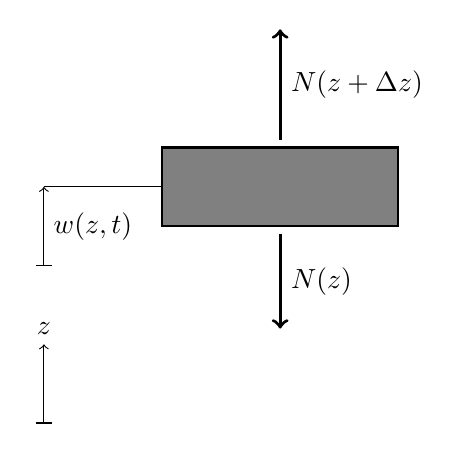
\begin{tikzpicture}
          \draw[thick, fill=gray] (-1.5,-0.5) rectangle (1.5,0.5);
          \draw[->] (-3,-3) -- (-3,-2) node[above] {$z$};
          \draw (-3.1,-3) --(-2.9,-3);
          \draw[->] (-3,-1) -- node[right] {$w(z,t)$} (-3,0);
          \draw (-3.1,-1) --(-2.9,-1);
          \draw (-3,0) -- (-1.5,0);
          \draw[->, very thick] (0, 0.6) -- node[right] {$N(z+\Delta z)$} (0, 2);
          \draw[->, very thick] (0,-0.6) -- node[right] {$N(z)$} (0,-1.8);
\end{tikzpicture}
 

 \end{column}
        \begin{column}[t]{.5\linewidth}
        \vspace{-5cm}
        \begin{align*}
         \rho A \Delta z \ddot{w}&=N(z+\Delta z) - N(z)  \\
         \rho A \Delta z \ddot{w}&=EAw'(z+\Delta z) - EAw'(z)  \\
         \rho \ddot{w}&=Ew''  
        \end{align*}
        Wellengleichung (hyperbolische PDE)
        \begin{equation*}
         \ddot{w}=c^2 w''
        \end{equation*}
        mit $c^2=E/\rho$, $\dot{w}=\frac{\partial w}{\partial t}$ und $w'=\frac{\partial w}{\partial z}$.
        \end{column}
        
 \end{columns}
\end{frame}


\begin{frame}
\frametitle{D'Alembertscher Wellenansatz 1/5}
Kanonische Koordinaten 
\hfill 
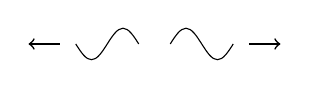
\begin{tikzpicture}
\draw[->, semithick] (-1.2, 0) -- (-1.6, 0);
\draw (-0.2, 0) sin (-0.4, 0.2) cos (-0.6, 0) sin (-0.8,-0.2) cos (-1.0, 0);
\draw ( 0.2, 0) sin ( 0.4, 0.2) cos ( 0.6, 0) sin ( 0.8,-0.2) cos ( 1.0, 0);
\draw[->, semithick] ( 1.2, 0) -- (1.6, 0);
\end{tikzpicture}

\begin{align*}
 \xi &= z+ct \\
 \eta &= z-ct 
\end{align*}
damit $w\bigl( \xi(z,t), \eta(z,t) \bigr)$ und die Ableitungen
\begin{align*}
\frac{\partial w}{\partial z} &= \frac{\partial w}{\partial \xi} + \frac{\partial w}{\partial \eta} \\
\frac{\partial^2 w}{\partial z^2} &= \frac{\partial^2 w}{\partial \xi^2} +
2\frac{\partial^2 w}{\partial \xi \partial \eta} + \frac{\partial^2 w}{\partial \eta^2} \\
\frac{\partial w}{\partial t} &=c\left( \frac{\partial w}{\partial \xi} - \frac{\partial w}{\partial \eta}\right) \\
\frac{\partial^2 w}{\partial t^2} &= c^2\left( \frac{\partial^2 w}{\partial \xi^2} -2\frac{\partial^2 w}{\partial \xi \partial \eta} + \frac{\partial^2 w}{\partial \eta^2}\right)
\end{align*}
\end{frame}

\begin{frame}
\frametitle{D'Alembertscher Wellenansatz 2/5}
Einsetzen in die Wellengleichung ergibt
\begin{equation*}
 \frac{\partial^2 w}{\partial \xi \partial \eta}=0
\end{equation*}
und anschließende Integration nach $\xi$ und dann nach $\eta$ führt zu
\begin{align*}
 \frac{\partial w}{\partial \eta} &= \phi(\eta) \\
 w&=\Phi(\eta) + \Psi(\xi).
\end{align*}
Die allgemeine Lösung der Wellengleichung besteht aus ``einer nach rechts'' und ``einer nach links laufenden'' Funktion. 
\end{frame}

\begin{frame}
\frametitle{D'Alembertscher Wellenansatz 3/5}
Um die Funktionen zu bestimmen, sind die Anfangsbedingungen, einfachheitshalber zu $t=0$, auszuwerten
\begin{align*}
 w_0(z)&=\Psi(z)+\Phi(z),\\
 \dot{w}_0(z)&=c\Psi'(z)-c\Phi'(z),
\end{align*}
oder nach Integration der zweiten Gleichung
\begin{align*}
 w_0(z)&=\Psi(z)+\Phi(z),\\
 \int_{z_0}^z  \dot{w}_0(\bar{z})\,\mathrm{d}\bar{z}+K&=c\Psi(z)-c\Phi(z),
\end{align*}
Dieses Gleichungssystem lässt sich algebraisch nach den gesuchten Funktionen auflösen.
\end{frame}

\begin{frame}
\frametitle{D'Alembertscher Wellenansatz 4/5}
\begin{align*}
 \Phi(z)&=\frac{1}{2}w_0(z)-\frac{1}{2c} \int_{z_0}^z  \dot{w}_0(\bar{z})\,\mathrm{d}\bar{z},\\
 \Psi(z)&=\frac{1}{2}w_0(z)+\frac{1}{2c} \int_{z_0}^z  \dot{w}_0(\bar{z})\,\mathrm{d}\bar{z},\\
\end{align*}
und zurück in den Originalkoordinaten
\begin{equation*}
 w(z,t)=\frac{1}{2}\Bigl( w_0(z-ct) + w_0(z+ct) \Bigr)+\frac{1}{2c} \int_{z-ct}^{z+ct}  \dot{w}_0(\bar{z})\,\mathrm{d}\bar{z}.
\end{equation*}
\end{frame}

\begin{frame}
\frametitle{D'Alembertscher Wellenansatz 5/5}

\only<1>{
\begin{center}
\begin{tikzpicture}
\draw[->] (-1,0) -- (10, 0) node[right] {$z$};
\draw[->] (0,-0.5) -- (0, 5) node[above] {$t$};
\fill (5, 0) circle[radius=0.05];
\draw (5, 0) node[below] {$z_0$};
\draw (5, 0) -- (1,4) node[above] {$z=z_0-ct$};
\draw (5, 0) -- (9,4) node[above] {$z=z_0+ct$};
\end{tikzpicture}

Einflussbereich
\end{center}
}

\only<2>{
\begin{center}
\begin{tikzpicture}
\draw[->] (-1,0) -- (10, 0) node[right] {$z$};
\draw[->] (0,-0.5) -- (0, 5) node[above] {$t$};
\fill (5, 4) circle[radius=0.05];
\draw (5, 0) node[below] {$z_1$};
\draw (0, 4) node[left] {$t_1$};
\draw (5, 4) -- (2,1) node[below] {$z=z_1+c(t-t_1)$};
\draw (5, 4) -- (8,1) node[below] {$z=z_1-c(t-t_1)$};
\draw (-0.1, 4) -- (0.1, 4);
\draw (5, -0.1) -- (5, 0.1);
\end{tikzpicture}

Abhängigkeitsintervall
\end{center}
}

\end{frame}

\begin{frame}
\frametitle{Beispiel}
\only<1>{
\begin{center}
Anfangsbedingungen: \quad
$w_0(z)=\left\{\begin{array}{ll}
      1,& z\in[-1,1]\\
      0,& \text{otherwise}
     \end{array} \right.$, \qquad
$\dot{w}_0(z)=0$

\vspace{-4cm}

\begin{animateinline}[draft, autoplay, loop]{10}
    \multiframe{30}{rDKtime=0.0+1}{   % number of frames, parameter (i-integer, r-real, d-dimension) =  initial value + increment
\begin{tikzpicture}[scale=2, domain=-5:5, samples=100]
\tikzmath{\DKpos=0.1*(sign(\rDKtime-5)+1)*\rDKtime;}
\draw[->] (-5.2,0) -- (5.2,0) node[right] {$z$};
\draw[->] (0,-0.2) -- (0,2.2) node[above] {$w$};
\draw plot (\x,{0.5*sign(\x+1+\DKpos)-0.5*sign(\x-1+\DKpos)+0.5*sign(\x+1-\DKpos)-0.5*sign(\x-1-\DKpos)});
\end{tikzpicture}
}
\end{animateinline}

\end{center}
}

\only<2>{
\begin{center}
\begin{tikzpicture}
\draw[->] (-5.5,0) -- (5.5, 0) node[right] {$z$};
\draw[->] (0,-0.5) -- (0, 5) node[above] {$t$};
\draw (-1, 0) -- (-5,5);
\draw (-1, 0) -- ( 3,5);
\draw ( 1, 0) -- (-3,5);
\draw ( 1, 0) -- ( 5,5);
\draw ( 1, 0.1) -- ( 1,-0.1) node[below] {$1$};
\draw (-1, 0.1) -- (-1,-0.1) node[below] {$-1$};
\end{tikzpicture}

Lösungsbereiche im $z$-$t$-Diagramm
\end{center}
}

\end{frame}



\begin{frame}
 \frametitle{Energietransport}
Energiebilanz eines endlichen Abschnitts $[z_1, z_2]$ 
\begin{equation*}
 \frac{\mathrm{d}}{\mathrm{d}t} \bigl( E_\mathrm{kin}+E_\mathrm{pot} \bigr)=P(z_1,t)-P(z_2,t)
\end{equation*}
\only<1>{
\begin{align*}
E_\mathrm{kin}&= \int_{z_1}^{z_2}\frac{1}{2}\rho A \dot{w}^2\,\mathrm{d}z\\
\frac{\mathrm{d}E_\mathrm{kin}}{\mathrm{d}t}&= \int_{z_1}^{z_2}\rho A \dot{w}\ddot{w}\,\mathrm{d}z=\int_{z_1}^{z_2} EA \dot{w} w'' \,\mathrm{d}z\\
E_\mathrm{pot}&= \int_{z_1}^{z_2}\frac{1}{2}E A w'^2\,\mathrm{d}z\\
   \frac{\mathrm{d}E_\mathrm{pot}}{\mathrm{d}t}&=\int_{z_1}^{z_2} EA w'\dot{w}'\,\mathrm{d}z
\end{align*}
}

\only<2>{
\begin{align*}
\frac{\mathrm{d}}{\mathrm{d}t} \bigl( E_\mathrm{kin}+E_\mathrm{pot} \bigr)&=
EA\int_{z_1}^{z_2}\dot{w} w'' + w'\dot{w}'\,\mathrm{d}z\\
&= EA\left|\dot{w}w'\right|_{z_1}^{z_2}+
EA\int_{z_1}^{z_2}-\dot{w}' w' + w'\dot{w}'\,\mathrm{d}z\\
&=EA\left|\dot{w}w'\right|_{z_1}^{z_2}
\end{align*}
Der Vergleich mit der Energiebilanz zeigt
\begin{equation*}
 P(z,t)= -EA w'(z,t)\dot{w}(z,t)=EAc\left( \left(\frac{\partial \Phi(\eta)}{\partial \eta}\right)^2 - \left(\frac{\partial \Psi(\xi)}{\partial \xi}\right)^2 \right)
\end{equation*}
}

\end{frame}



\begin{frame}
\hspace{1cm} \frametitle{Halbunendlicher Stab 1/3}
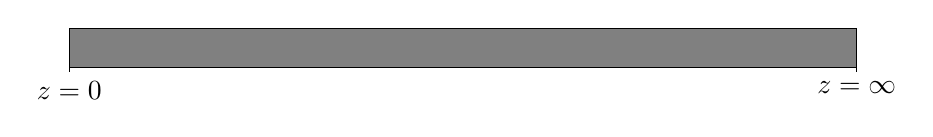
\begin{tikzpicture}
\draw[fill=gray] (0, 0) rectangle (10, 0.5);
\draw ( 0, 0) -- ( 0, -0.05) node[below] {$z=0$};
\draw (10, 0) -- (10, -0.05) node[below] {$z=\infty$};
\end{tikzpicture}

\begin{align*}
 \Phi(z)&=\frac{1}{2}w_0(z)-\frac{1}{2c} \int_{z_0}^z  \dot{w}_0(\bar{z})\,\mathrm{d}\bar{z},\\
 \Psi(z)&=\frac{1}{2}w_0(z)+\frac{1}{2c} \int_{z_0}^z  \dot{w}_0(\bar{z})\,\mathrm{d}\bar{z},\\
\end{align*}
Für den halbunendlichen Stab brauchen wir
\begin{align*}
 \Phi(z-ct) & &\text{für alle}& &-\infty &< z-ct < \infty & &\\ %rechtslaufend
 \Psi(z+ct) & &\text{für alle}& & 0 &< z+ct < \infty & &%linkslaufend
\end{align*}
Für $z-ct\ge 0$ greifen wir auf bekannte Anfangsbedingungen zurück und erhalten die D'Alembertsche Lösung, wie für den unendlichen Stab.
%modifizierter D'Alembert [SF]
\end{frame} 

\begin{frame}
\frametitle{Halbunendlicher Stab 2/3}
Im anderen Fall $z-ct<0$ nutzen wir die Randbedingung 
\begin{equation*}
 w(0,t)=\Phi(0-ct)+\Psi(0+ct)=0
\end{equation*}
und erkennen eine \textsl{Spiegelung}
\begin{equation*}
 \Phi(-ct)=-\Psi(ct).
\end{equation*}
Weil diese Beziehung für alle Zeiten $t$ gilt, lässt sich folgende Ersetzung durch bekannte Größen durchführen
\begin{equation*}
\Phi(\underbrace{z-ct}_{<0})=-\Psi(\underbrace{-z+ct}_ {>0}). 
\end{equation*}
\end{frame}

\begin{frame}
\frametitle{Halbunendlicher Stab 3/3}
Damit lautet das Endergebnis ``modifizierte D'Alembertsche Lösung''
\begin{equation*}
 w(z,t)=\left\{ \begin{array}{ll}
                 \frac{1}{2}\Bigl( w_0(z-ct) + w_0(z+ct) \Bigr)+\frac{1}{2c} \int_{z-ct}^{z+ct}  \dot{w}_0(\bar{z})\,\mathrm{d}\bar{z}, & z \ge ct, \\
                 \frac{1}{2}\Bigl( -w_0(-z+ct) + w_0(z+ct) \Bigr)+\frac{1}{2c} \int_{-z+ct}^{z+ct}  \dot{w}_0(\bar{z})\,\mathrm{d}\bar{z}, & z < ct. 
                \end{array}
  \right.
\end{equation*}
\begin{tikzpicture}
\draw[->] (-1,0) -- (11.5, 0) node[right] {$z$};
\draw[->] (0,-0.25) -- (0, 3) node[above] {$t$};
\draw[dashed] (0, 0) -- (7.5, 2.5) node[above] {$z=ct$};
\fill[color=gray] (4, 1) circle[radius=0.05];
\draw[->] (1, 0) -- (4,1);
\draw[->] (8, 0) -- (4,1);
\fill[color=gray] (4, 2) circle[radius=0.05];
\draw[->] (2, 0) -- (0, 0.667) -- (4,2);
\draw[->] (11, 0) -- (4,2);
\end{tikzpicture}

\end{frame}

\begin{frame}
 \frametitle{Häufige Randbedingungen}

\begin{itemize}
 \item vorgeschriebene Verschiebung \quad $w(z_\mathrm{R},t)=w_\mathrm{R}(t)$
 \item vorgeschriebene Kraft \qquad $EA w'(z_\mathrm{R},t)=F_\mathrm{R}(t)$
\end{itemize}

\bigskip

\only<1>{
fester Rand $w(0,t)=0$
\begin{center}
\vspace{-6cm}
\begin{animateinline}[draft, autoplay, loop]{10}
    \multiframe{40}{rDKtime=0.0+1}{   % number of frames, parameter (i-integer, r-real, d-dimension) =  initial value + increment
\begin{tikzpicture}[scale=2, domain=-5:5, samples=50]
\tikzmath{\DKpos=6-0.33*\rDKtime;}
\draw[dashed] (-5.5,0) -- (0, 0);
\draw[->]  (0, 0) -- (5.5, 0) node[right] {$z$};
\draw[->] (0,-1.1) -- (0, 2.5) node[above] {$w$};
\draw plot (\x,{0.5*sign(\x+1-\DKpos)-0.5*sign(\x-1-\DKpos)-0.5*sign(\x+1+\DKpos)+0.5*sign(\x-1+\DKpos)});
\end{tikzpicture}
}
\end{animateinline}

\end{center}
}

\only<2>{
freier Rand $w'(0,t)=0$
\begin{center}
\vspace{-6cm}
\begin{animateinline}[draft, autoplay, loop]{10}
    \multiframe{40}{rDKtime=0.0+1}{   % number of frames, parameter (i-integer, r-real, d-dimension) =  initial value + increment
\begin{tikzpicture}[scale=2, domain=-5:5, samples=50]
\tikzmath{\DKpos=6-0.33*\rDKtime;}
\draw[dashed] (-5.5,0) -- (0, 0);
\draw[->] (0,0) -- (5.5, 0) node[right] {$z$};
\draw[->] (0,-1.1) -- (0, 2.5) node[above] {$w$};
\draw plot (\x,{0.5*sign(\x+1-\DKpos)-0.5*sign(\x-1-\DKpos)+0.5*sign(\x+1+\DKpos)-0.5*sign(\x-1+\DKpos)});
\end{tikzpicture}
}
\end{animateinline}

\end{center}
}

\end{frame} 


\begin{frame}
 \frametitle{Übergangsbedingungen 1/3}
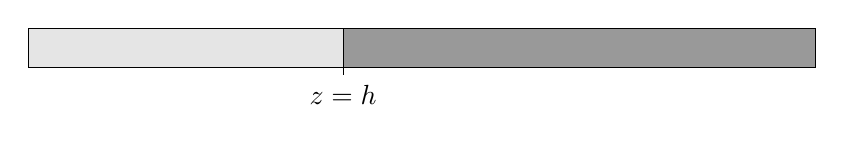
\begin{tikzpicture}
\draw[fill=black!10] (0, 0) rectangle (4, 0.5);
\draw[fill=black!40] (4, 0) rectangle (10, 0.5);
\draw ( 4, 0) -- ( 4, -0.1) node[below] {$z=h$};
\end{tikzpicture}

 
Kinematische ($\dot{w}(h^-)=\dot{w}(h^+)$) und kinetische Kontinuität ($N(h^-)=N(h^+)$) an der Stelle $z=h$
\begin{align*}
 -c_1\Phi_1'(z-c_1t) + c_1\Psi_1'(z+c_1t) &= -c_2\Phi_2'(z-c_2t),  \\
 E_1A_1\Phi_1'(z-c_1t) + E_1A_1 \Psi_1'(z+c_1t) &= E_2A_2\Phi_2'(z-c_2t).
\end{align*}
Aufgelöst nach reflektierter und transmittierter Welle
\begin{align*}
 \Psi_1' &= \frac{c_2/c_1 - E_2 A_2/(E_1 A_1)}{c_2/c_1+ E_2 A_2/(E_1 A_1)}\Phi_1',\\
 \Phi_2' &= \frac{2}{c_2/c_1 + E_2 A_2/(E_1 A_1)}\Phi_1'.\\
\end{align*}
\end{frame} 


\begin{frame}
 \frametitle{Übergangsbedingungen 2/3}
  Für einen Stab konstanter Querschnittsfläche $A_1=A_2=A$ lauten die Schnelleverhältnisse
  \begin{align*}
   R_v&=\frac{c_1\Psi_1'}{-c_1\Phi_1'}=\frac{\rho_1 c_1 - \rho_2 c_2}{\rho_1 c_1 + \rho_2 c_2}, \\
   T_v&= \frac{-c_2\Phi_2'}{-c_1\Phi_1'}=\frac{2\rho_1 c_1}{\rho_1 c_1 + \rho_2 c_2 },
  \end{align*}
und die Spannungsverhältnisse
\begin{align*}
   R_\sigma &= \frac{E_1\Psi_1'}{E_1\Phi_1'}=-\frac{\rho_1 c_1 - \rho_2 c_2}{\rho_1 c_1 + \rho_2 c_2}, \\
   T_\sigma &= \frac{E_2\Phi_2'}{E_1\Phi_1'}=\frac{2\rho_2 c_2}{\rho_1 c_1 + \rho_2 c_2 }.
\end{align*}  
\end{frame} 

\begin{frame}
 \frametitle{Übergangsbedingungen 3/3}
Der Grenzfall sehr kleiner Steifigkeit des anschließenden Abschnitts nähert sich einer Reflexion am freien Rand
\begin{align*}
 \lim_{c_2 \to 0} R_v &= 1, \\
 \lim_{c_2 \to 0} R_\sigma &= -1,
\end{align*}
und im Grenzfall sehr hoher Steifkeit einer Reflexion am festen Rand
\begin{align*}
 \lim_{c_2 \to \infty} R_v &= -1 , \\
 \lim_{c_2 \to \infty} R_\sigma &= 1.
\end{align*}
\end{frame} 

\begin{frame}
 \frametitle{Beispiel}
\begin{figure}
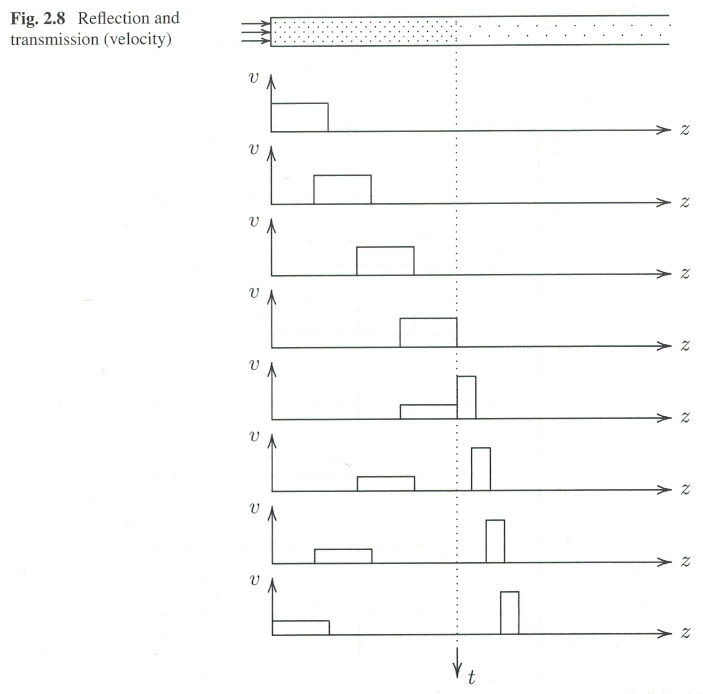
\includegraphics[width=0.475\textwidth]{fig_pdf/transition_z_v}
\hfill
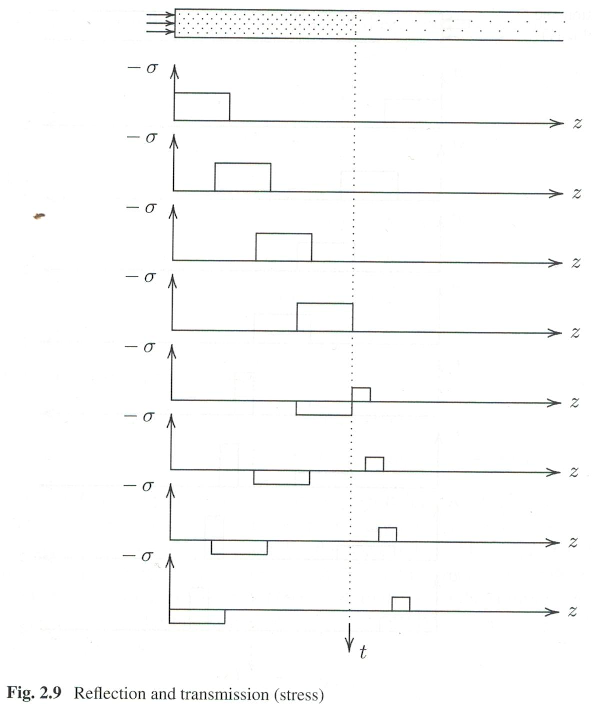
\includegraphics[width=0.4\textwidth]{fig_pdf/transition_z_sigma}
\caption*{$E_1=9E_2$, $A_1=A_2$, $\rho_1=\rho_2$ \cite{Verruijt2010}}
\end{figure}
\end{frame} 


\begin{frame}
 \frametitle{Diskrete Elemente}
 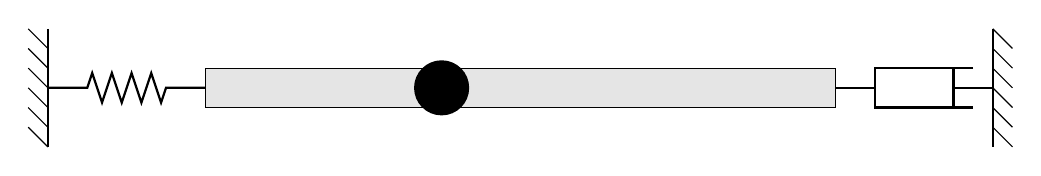
\begin{tikzpicture}
\draw (0, 0.25) pic [scale=0.5] {DKbase};
\draw (0, 0.25) pic [scale=0.5, thick] {DKspring=4};  
\draw[fill=black!10] (2, 0) rectangle (10, 0.5);
\draw (10, 0.25) pic [scale=0.5, thick] {DKdashpot=4};
\draw (12, 0.25) pic [scale=0.5, rotate=180] {DKbase};
\fill (5, 0.25) circle [radius=0.35];
 \end{tikzpicture}


 \begin{itemize}
  \item Feder;
  \item Masse;
  \item Dämpfer, Anpassung $c=A\sqrt{E\rho}$.
 \end{itemize}
\hfill \dots \textsl{siehe Übung}.
\end{frame} 

%%%%%%%%%%%%%%%%%%%%%%%%%%%%%%%%%%%%%%%%%%%%%%%%

\section*{Literaturverzeichnis}

\begin{frame}[allowframebreaks]{}
	\printbibliography
\end{frame}
\end{document}
